\documentclass[12pt, a4paper]{report}
\usepackage{style}

\newcommand{\usecase}[9]{
    \def\arraystretch{1.5} 
    \vspace*{0.2cm}
    \begin{center}
        \begin{tabular}{|l|p{12cm}|}
            \hline
            \textbf{Actor(s)} & #4 \\
            \hline
            \textbf{Entry Condition} & #5 \\
            \hline
            \textbf{Event Flow} & #6 \\
            \hline
            \textbf{Exit Condition} & #7 \\
            \hline
            \textbf{Exceptions} & #8 \\
            \hline
            \textbf{Notes} & #9 \\
            \hline
        \end{tabular}
    \end{center}
    #1
}

\title{Software Engineering II\\ \textit{Exercises}}
\author{Christian Rossi}
\date{Academic Year 2023-2024}


\begin{document}

    \maketitle

    \begin{abstract}
    The course is structured around three main parts. 
    The first part focuses on approaches to Big Data management, addressing various challenges and dimensions associated with it.
    Key topics include the data engineering and data science pipeline, enterprise-scale data management, and the trade-offs between scalability, persistency, and volatility. 
    It also covers issues related to cross-source data integration, the implications of the CAP theorem, the evolution of transactional properties from ACID to BASE, as well as data sharding, replication, and cloud-based scalable data processing.

    The second part delves into systems and models for handling Big and unstructured data. It examines different types of databases, such as graph, semantic, columnar, document-oriented, key-value, and IR-based databases. 
    Each type is analyzed across five dimensions: data model, query languages, data distribution, non-functional aspects, and architectural solutions.
    
    The final part explores methods for designing applications that utilize unstructured data.
    It covers modeling languages and methodologies within the data engineering pipeline, along with schema-less, implicit-schema, and schema-on-read approaches to application design.
\end{abstract}

    \cleardoublepage
    \pagenumbering{Roman}

    \tableofcontents

    \cleardoublepage
    \pagenumbering{arabic}

    \chapter{Exercises session I}
    \section{Definition}

The realm of software engineering is dedicated to unraveling the multitude of challenges that emerge during the creation of extensive software systems.
These systems are inherently intricate due to their substantial scale, the collaboration of individuals from diverse fields, and the necessity for continuous adjustments to meet evolving demands (both during development and post-installation). 

\begin{definition}
    \emph{Software engineering} is a methodical and managerial discipline that revolves around the systematic creation and upkeep of software products, all of which are crafted and sustained within predefined, controlled timeframes and cost constraints.
\end{definition}

In contrast to traditional programming, where a programmer typically crafts an entire piece of software based on known specifications independently, software engineers embark on a distinct path.
They identify requirements, shape specifications, design components meant to interconnect with others, and engage in collaborative efforts within a team setting. 
The key competencies of a software engineer encompass technical acumen, managerial prowess, cognitive aptitude, and organizational skills.
    \section{Concurrent systems}

When transitioning from sequential to concurrent or parallel systems, fundamental shifts occur in how we define and model computation:
\begin{itemize}
    \item Usually, the traditional problem formulation changes significantly.
    \item The rise of networked and interactive systems demands new models focused on interactions rather than just algorithmic transformations.
    \item Many modern systems do not have a clear beginning and end but instead involve continuous, ongoing computations.
        This requires us to consider infinite sequences (infinite words), leading to a whole branch of formal language theory designed for such systems.
    \item We must account for interleaved signals flowing through different channels.
\end{itemize}
\begin{definition}[\textit{System}]
    A system is a collection of abstract machines, often referred to as processes.
\end{definition}
In some cases, we can construct a global state by combining the local states of individual processes. 
However, with concurrent systems, this is often inconvenient or even impossible:
\begin{itemize}
    \item Each process evolves independently, synchronizing only occasionally.
    \item Asynchronous systems do not have a globally synchronized state.
    \item Finite State Machines capture interleaving semantics but differ fundamentally from asynchronous models.
\end{itemize}
\noindent In distributed systems, components are physically separated and communicate via signals.
As system components operate at speeds approaching the speed of light, it becomes meaningless to assume a well-defined global state at any given moment.

\subsection{Time formalization}
When time becomes a factor in computation, things become significantly more complex. 
Unlike traditional engineering disciplines computer science often abstracts away from time, treating it separately in areas like complexity analysis and performance evaluation.

While this abstraction is sufficient for many applications, it is inadequate for real-time systems, where correctness explicitly depends on time behavior. 
In such systems, we must consider:
\begin{enumerate}
    \item The occurrence and order of events.
    \item The duration of actions and states.
    \item Interdependencies between time and data.
\end{enumerate}
Over the years, time has been integrated into formal models in various ways.

\paragraph*{Operational formalism}
These approaches incorporate time directly into system execution models: timed transitions, timed Petri networks, and time as a system variable. 

\paragraph*{Descriptive formalism}
These approaches focus on reasoning about time without explicitly simulating execution: temporal logic (treats time as an abstract concept, focusing on event ordering rather than durations), and metric temporal logics (extensions of temporal logic introduce time constraints).

    \chapter{Exercise session II}
    \section{Introduction}

Sensors serve to detect both the internal condition of the robot (proprioceptive sensors) and the external state of the environment (exteroceptive sensors).

Effectors are responsible for altering the state of the environment, with actuators facilitating the actions of effectors.
    \section{Linear regression}

The goal of regression is to approximate a function $f(x)$ that maps input $x$ to a continuous output $t$ from a dataset $\mathcal{D}$: 
\[\mathcal{D}=\left\{ \left\langle x,t \right\rangle \right\} \implies t=f(x)\]
Here, $x$ is a vector. 
To perform regression, we assume the existence of a function capable of performing this mapping.
The key components of constructing a linear regression problem include:
\begin{itemize}
    \item The method used to model the function $f$ (the hypothesis space). 
    \item The evaluation criteria for the approximation (the loss function).
    \item The optimization process for optimizing the model.
\end{itemize}

In linear regression, the function $f$ is modeled using linear functions. 
This choice is motivated by several factors:
\begin{itemize}
    \item Linear models are easily interpretable, making them suitable for explanation.
    \item Linear regression problems can be solved analytically, allowing for efficient computation.
    \item Linear functions can be extended to model nonlinear relationships.
    \item More sophisticated methods often build upon or incorporate elements of linear regression.
\end{itemize}

\paragraph*{Hypothesis space}
In mathematical terms, the approximation $y$ can be defined as: 
\[y(\textbf{x},\textbf{w})=w_0+\sum_{j=1}^{D-1}w_j x_j=\textbf{w}^T\textbf{x}\]
Here, $\textbf{x} = \left( 1,x_1,\dots,x_{D-1} \right)$ is a vector, and $w_0$ is called the bias parameter.
It's important to note that the output $y$ is a scalar value. 

In a two-dimensional space, our hypothesis space will be the set of all points in the plane $(w_0,w_1)$. 
The coordinates of each point will correspond to a line in the $\left( \textbf{x}, y \right)$ space.

\paragraph*{Loss function}
A commonly used error loss function for the linear regression problem is the sum of squared errors (SSE), defined as:
\[L(\textbf{w})=\dfrac{1}{2}\sum_{n=1}^{N}\left( y(x_n, \textbf{w})-t_n \right)^2\]
This sum is also referred to as the residual sum of squares (RSS) and can be expressed as the sum of squared residual errors:
\[RSS(\textbf{w})=\left\lVert \boldsymbol{\epsilon}^2_2 \right\rVert = \sum_{i=1}^{N}\epsilon^2_i \]
This formulation of the loss function allows for obtaining a closed-form optimization solution.

\paragraph*{Optimization}
For linear models, a closed-form optimization of the RSS, known as least squares, begins with the matrix representation of the loss function:
\[L(\textbf{w})=\dfrac{1}{2}RSS(\textbf{w})=\dfrac{1}{2}\left( \textbf{t}-\boldsymbol{\Phi}_{\textbf{w}} \right)^T\left( \textbf{t}-\boldsymbol{\Phi}_{\textbf{w}} \right)\]
Here, $\boldsymbol{\Phi}=\begin{bmatrix} \phi(x_1) & \dots & \phi(x_N)\end{bmatrix}^T$ and $\textbf{t}=\begin{bmatrix}t_1 & \dots & t_n\end{bmatrix}^T$.
To find the optimal $\textbf{w}$, we compute the first derivative of $L(\textbf{w})$ and set it to zero:
\[\hat{\textbf{w}}_{OLS}=\left( \boldsymbol{\Phi}^T\boldsymbol{\Phi}\right)^{-1}\boldsymbol{\Phi}^T\textbf{t}\]
However, the inversion of the matrix $\boldsymbol{\Phi}^T\boldsymbol{\Phi}^{-1}$ can be computationally expensive, especially for large datasets, with a complexity of $O(nm^2+m^3)$, assuming the matrix is non-singular (invertible). 

To mitigate this, stochastic gradient descent (SGD) can be employed. 
The algorithm known as least mean squares (LMS) uses the following update rule:
\[L(\textbf{x})=\sum_nL(x_n)\]
Expanding this, we get:
\begin{align*}
    \textbf{w}^{(n+1)}  &= \textbf{w}^{(n)}-\alpha^{(n)}\nabla L(x_n) \\
                        &= \textbf{w}^{(n)}-\alpha^{(n)}\left( \textbf{w}^{(n)^T}\phi(\textbf{x}_n)-t_n \right)\phi(\textbf{x}_n)
\end{align*}
Here, $\alpha$ is the learning rate, and convergence is guaranteed if $\sum_{n=0}^{\infty}=+\infty$ and $\sum_{n=0}^{\infty}=\alpha^{(n)^2}<+\infty$.

If the regression problem involves multiple outputs, meaning that $\textbf{t}$ is not a scalar, we can solve each regression problem independently.
However, we can still use the same set of basis functions.
The solution for the weight vectors for all outputs can be expressed as:
\[\hat{\textbf{W}}=\left( \boldsymbol{\Phi}^T\boldsymbol{\Phi}\right)^{-1}\boldsymbol{\Phi}^T\textbf{T}\]
Here, each column of matrix $\textbf{T}$ and $\hat{\textbf{W}}$ corresponds to the target vector and the weight vector for each output, respectively.
This solution can be easily decoupled for each output $k$: 
\[\hat{\textbf{w}}_k=\left( \boldsymbol{\Phi}^T\boldsymbol{\Phi}\right)^{-1}\boldsymbol{\Phi}^T\textbf{t}_k\]
An advantage of this approach is that $\left( \boldsymbol{\Phi}^T\boldsymbol{\Phi}\right)^{-1}$ only needs to be computed once, regardless of the number of outputs.

\subsection{Basis function}
While a linear combination of input variables may not always suffice to model data, we can still construct a regression model that is linear in its parameters. 
This can be achieved by defining a model using non-linear basis functions, expressed as:
\[y(\textbf{x},\textbf{w})=w_0+\sum_{j=1}^{M-1}w_j \phi_j(\textbf{x})=\textbf{w}^T\boldsymbol{\phi}(\textbf{x})\]
Here, the components of the vector  $\boldsymbol{\phi}(\textbf{x})=\left( 1,\phi_1(\textbf{x}),\dots,\phi_{M-1}(\textbf{x}) \right)^T$  are referred to as features.
These features allow for a more flexible representation of the input data, enabling the model to capture non-linear relationships between the input variables and the output.
\begin{example}
    Let's reconsider a set of data regarding individuals' weight and height, along with their completion times for a one-kilometer run:
    \begin{table}[H]
        \centering
        \begin{tabular}{c|c|c}
        \textbf{Height (cm)} & \textbf{Weight (kg)} & \textbf{Completion time (s)} \\ \hline
        180                  & 70                   & 180                          \\
        184                  & 80                   & 220                          \\
        174                  & 60                   & 170                         
        \end{tabular}
    \end{table}
    We can model this problem using a dummy variable and introduce the Body Mass Index (BMI) as a new feature:
    \begin{table}[H]
        \centering
        \begin{tabular}{c|c|c|c|c}
        \textbf{Dummy variable} & \textbf{Height (cm)} & \textbf{Weight (kg)} & \textbf{BMI} & \textbf{Completion time (s)} \\ \hline
        $x_0$                   & $x_1$                & $x_2$                & $x_3$        & $t$                          \\
        1                       & 180                  & 70                   & 21           & 180                          \\
        1                       & 184                  & 80                   & 23           & 220                          \\
        1                       & 174                  & 60                   & 20           & 170                         
        \end{tabular}
    \end{table}
    Here, the dummy variable $x_0$ is always initialized to one.
    Now, we have the option to retain or discard the weight and height variables, considering only the BMI values for analysis.
\end{example}
The most commonly used basis functions in regression are:
\begin{itemize}
    \item \textit{Polynomial}: 
        \[\phi_j(x)=x^j\]
    \item \textit{Gaussian}:
        \[\phi_j(x)=\exp \left( -\dfrac{\left( x-\mu_j \right)^2}{2 \sigma^2} \right) \]
    \item \textit{Sigmoidal}: 
        \[\phi_j(x)=\dfrac{1}{1+\exp\left(\dfrac{\mu_j-x}{\sigma}\right)}\]
\end{itemize}
Here, the constant $\mu_j$ is referred to as a hyperparameter, as its value needs to be determined through experimentation and depends on the user's experience.

\begin{figure}[H]
    \centering
    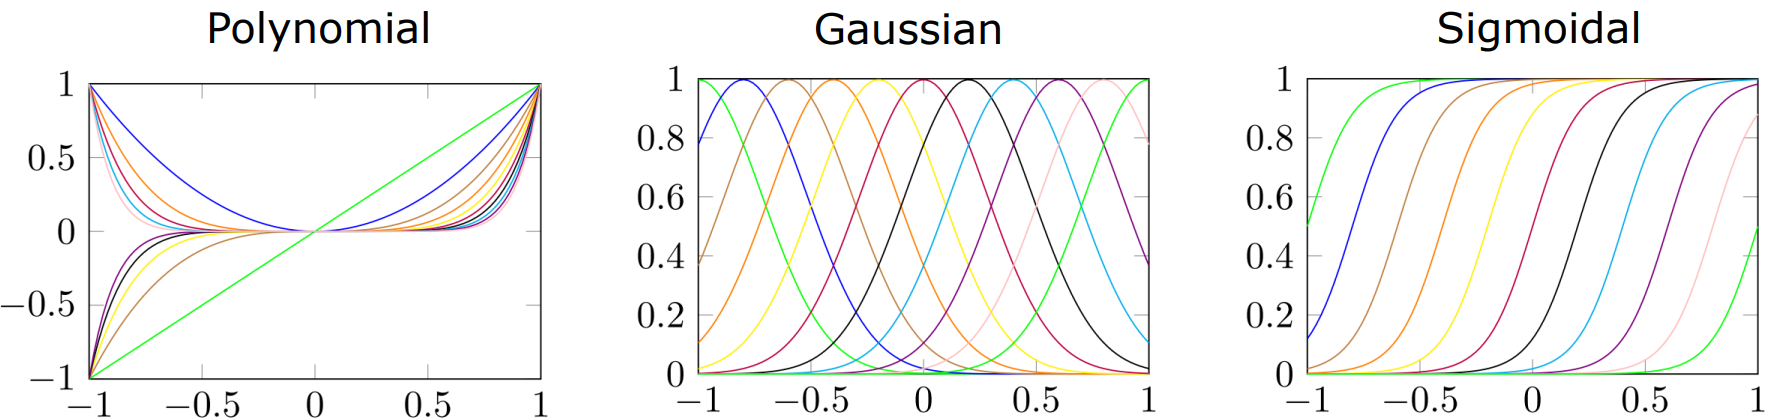
\includegraphics[width=0.75\linewidth]{images/basis.png}
    \caption{Some possible basis functions shapes}
\end{figure}

It's noteworthy that the Gaussian basis function allows for a local approximation by omitting values that are close to zero.
This approach enables capturing the relationship between the input and output in a reduced input space area.
As we move away from the mean, approaching zero, the values become negligible.

\subsection{Regularization}
A function can achieve a better approximation by increasing the degree of the polynomial used in the regression.
\begin{example}
    Consider a function generating a set of points with some noise:
    \begin{figure}[H]
        \centering
        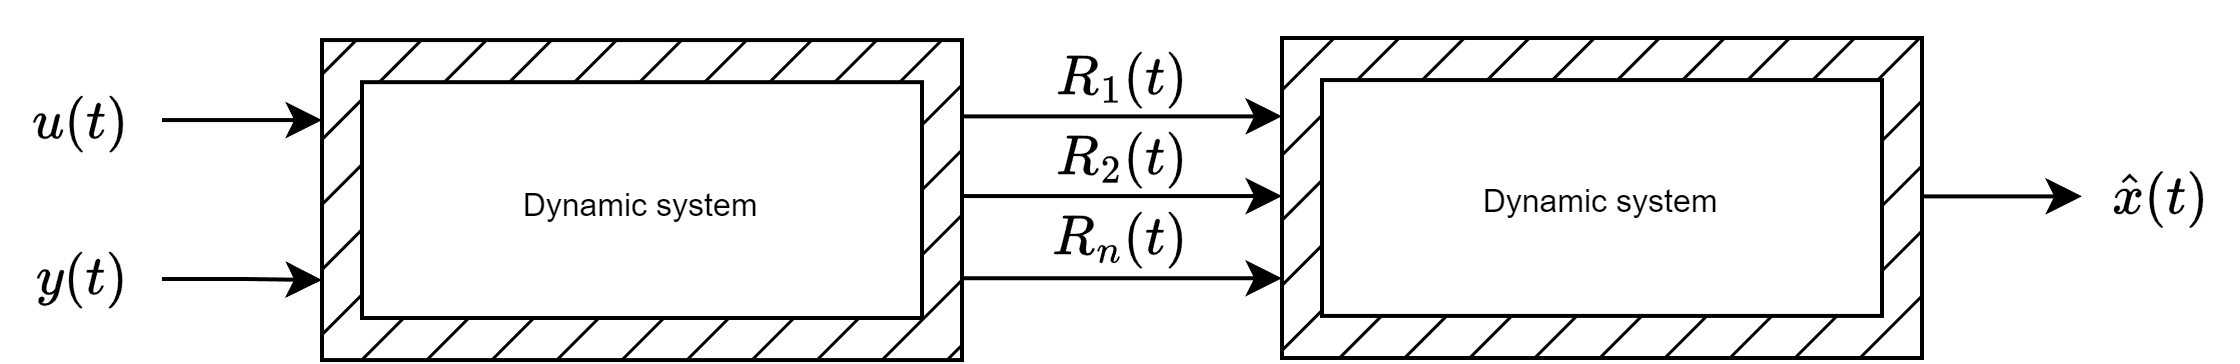
\includegraphics[width=0.25\linewidth]{images/reg.png}
    \end{figure}
    Using a second-order polynomial instead of a linear one provides a better approximation:
    \begin{figure}[H]
        \centering
        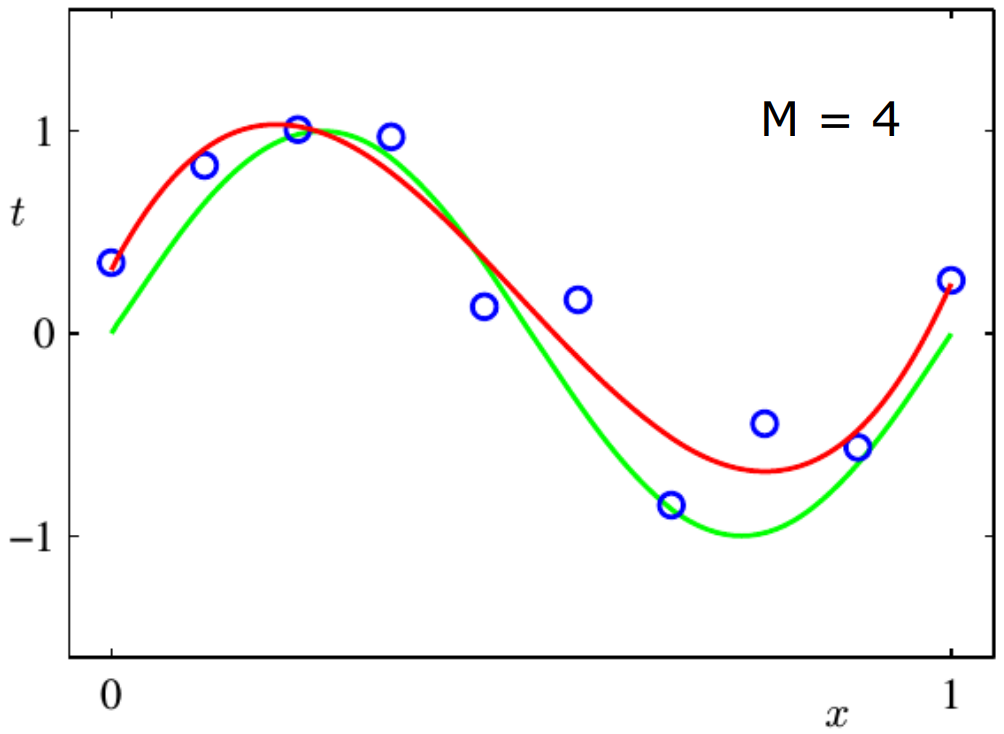
\includegraphics[width=0.25\linewidth]{images/reg1.png}
    \end{figure}
    Further improving the approximation can be achieved with a higher-degree polynomial (e.g., ninth grade):
    \begin{figure}[H]
        \centering
        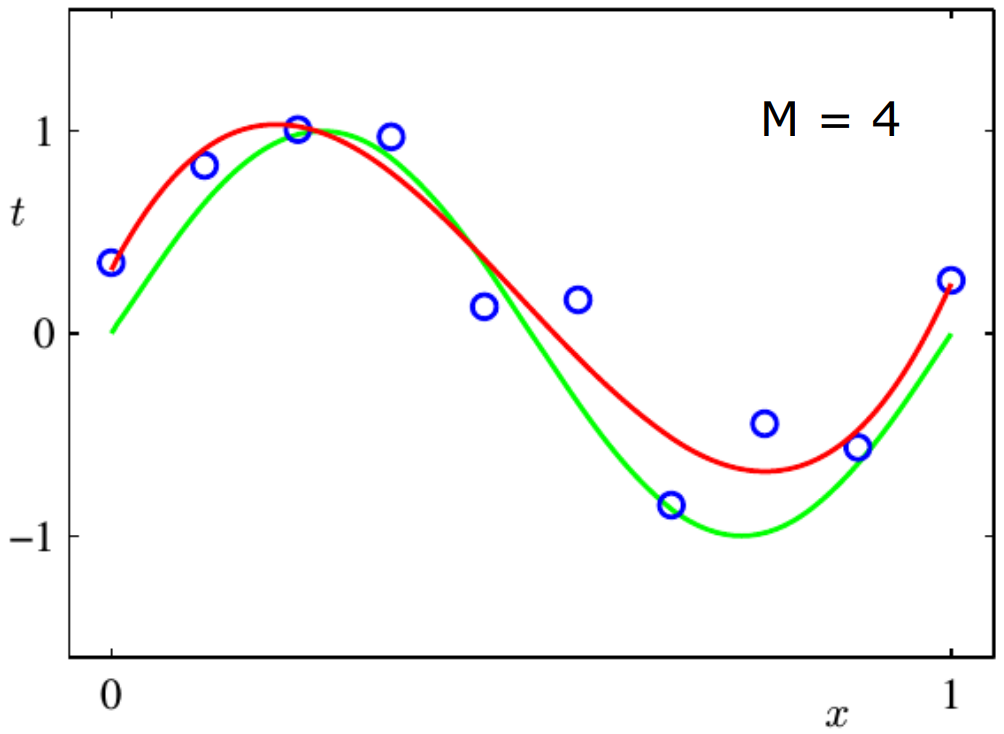
\includegraphics[width=0.25\linewidth]{images/reg1.png}
    \end{figure}
\end{example}
However, increasing the polynomial degree also increases the complexity of the model parameters.
To address this complexity, adjustments are needed in the loss function:
\[L(\textbf{w})=L_D(\textbf{w})+\lambda L_W(\textbf{w})\]
Here, $L_D(\textbf{w})$ represents the usual loss function, $L_W(\textbf{w})$ reflects model complexity (a hyperparameter), and $\lambda$ is the regularization coefficient.
$L_W(\textbf{w})$ can be tailored using ridge regression or lasso methods.

\paragraph*{Ridge regression}
In ridge regression, the regularization term $L_W(\textbf{w})$ is defined as:
\[L_W(\textbf{w})=\dfrac{1}{2}\textbf{w}^T\textbf{w}=\dfrac{1}{2}\left\lVert \textbf{w} \right\rVert_2^2 \]
Thus, the overall loss function becomes:
\[L(\textbf{w})=\dfrac{1}{2}\sum_{i=1}^N \left( t_i-\textbf{w}^T\phi(x_i) \right)^2 + \dfrac{\lambda}{2}\left\lVert \textbf{w} \right\rVert_2^2\]
Despite the regularization term, the loss function remains quadratic with respect to $w$, allowing for closed-form optimization:
\[\hat{\textbf{w}}_{ridge}=\left( \lambda\textbf{I}+\boldsymbol{\Phi}^T \boldsymbol{\Phi} \right)^{-1}\boldsymbol{\Phi}^T\text{t}\]
The term $\lambda\textbf{I}$ is crucial in solving the singularity problem, as it transforms a non-singular matrix into a singular one with an appropriate choice of $\lambda$. 

\paragraph*{Lasso}
Another common regularization method is lasso, where the regularization term $L_W(\textbf{w})$ is defined as:
\[L_W(\textbf{w})=\dfrac{1}{2}\left\lVert \textbf{w} \right\rVert_1=\dfrac{1}{2}\sum_{j=0}^{M-1}\left\lvert w_j \right\rvert\]
Thus, the overall loss function becomes:
\[L(\textbf{w})=\dfrac{1}{2}\sum_{i=1}^N \left( t_i-\textbf{w}^T\phi(x_i) \right)^2 + \dfrac{\lambda}{2}\left\lVert \textbf{w} \right\rVert_1\]
In this case, closed-form optimization is not possible. 
However, lasso typically leads to sparse regression models: when the regularization coefficient $\lambda$ is large enough, some components of $\hat{\textbf{w}}$ become equal to zero.
Regularization can be seen as equivalent to minimizing  $L_D(\textbf{w})$ subject to the constraint:
\[\sum_{j=0}^{M-1}\left\lvert w_j \right\rvert \leq \eta\] 

\subsection{Linear regression with probability}
We can approach regression in a probabilistic manner by defining a model that probabilistically maps inputs ($x$) to outputs ($t$).
This model, denoted as $y(x, w)$, incorporates unknown parameters ($w$).
We then model the likelihood, i.e., the probability that observed data $\mathcal{D}$ is generated by a given set of parameters ($w$), as: 
\[\text{P}(\mathcal{D}|\textbf{w})\]
Finally, we estimate the parameters ($w$) by maximizing the likelihood:
\[\textbf{w}_{ML}=\argmax_{\textbf{w}}\text{P}(\mathcal{D}|\textbf{w})\]

For linear regression, we define the model as:
\[t=y(\textbf{x},\textbf{w})+\epsilon=\textbf{w}^T\boldsymbol{\Phi}(\textbf{x})+\epsilon\]
Here, we assume a linear model for $y(\textbf{x},\textbf{w})$ and introduce noise  $\epsilon\sim\mathcal{N}(0,\sigma^2)$. 
Consequently, given a dataset $\mathcal{D}$ of $N$ samples with inputs $\textbf{X}=\begin{bmatrix}\textbf{x}_1 & \dots & \textbf{x}_n \end{bmatrix}$ and outputs $\textbf{t}=\begin{bmatrix}t_1 & \dots & t_n \end{bmatrix}^T$, we have: 
\[\text{P}(\mathcal{D}|\textbf{w})=\text{P}(\textbf{t}|\textbf{X},\textbf{w},\sigma^2)=\prod_{n=1}^{N}\mathcal{N}(t_n|\textbf{w}^T\boldsymbol{\Phi}(\textbf{x}_n),\sigma^2)\]
 
To find $\textbf{w}_{ML}$, it is convenient to maximize the log-likelihood, obtaining:
\[\ell (\textbf{w})=\ln\text{P}(t_n|\textbf{x}_n, \textbf{w} ,\sigma^2)=-\dfrac{N}{2}\ln(2\pi\sigma^2)-\dfrac{1}{2\sigma^2}RSS(\textbf{w})\]
Notice that the first part of the final formula is a constant independent of $\textbf{w}$, so it can be ignored in maximizing the likelihood.
Solving the optimization problem by setting the gradient to zero $\ell (\textbf{w})=0$, yields the final formula:
\[\textbf{w}_{ML}=\left( \boldsymbol{\Phi}^T\boldsymbol{\Phi} \right)^{-1}\boldsymbol{\Phi}^T\textbf{t}\]
This result aligns with the ordinary least squares approach.

This outcome allows us to interpret ordinary least squares from a probabilistic perspective, confirming that we are utilizing a normally distributed probabilistic function to generate the residuals in OLS.

\paragraph*{Bayesian linear regression}
Bayesian linear regression follows a structured approach:
\begin{enumerate}
    \item Formulation of probabilistic knowledge:
        \begin{enumerate}
            \item Qualitatively define the model expressing our knowledge.
            \item Incorporate unknown parameters into the model.
            \item Represent assumptions about these parameters with a prior distribution before observing any data.
        \end{enumerate}
    \item Data observation.
    \item Computation of posterior probability distribution for parameters:
        \[\text{P}(parameters|data)=\dfrac{\text{P}(data|parameters)\text{P}(parameters)}{\text{P}(data)}\]
    \item Utilization of Posterior Distribution to:
        \begin{itemize}
            \item Make predictions by averaging over the posterior distribution.
            \item Assess or accommodate uncertainty in parameter values.
            \item Make decisions by minimizing expected posterior loss.
        \end{itemize}
\end{enumerate}

The posterior distribution for model parameters is derived by combining the prior with the likelihood for parameters given the data:
\[\text{P}(\textbf{w}|\mathcal{D})=\dfrac{\text{P}(\mathcal{D}|\textbf{w})\text{P}(\textbf{w})}{\text{P}(\mathcal{D})}\]
Here, $\text{P}(\textbf{w})$ represents the prior probability over parameters, $\text{P}(\mathcal{D}|\textbf{w})$ denotes the likelihood, and $\text{P}(\mathcal{D})$ is the marginal likelihood acting as a normalization constant: 
\[\text{P}(\mathcal{D})=\int\text{P}(\mathcal{D}|\textbf{w})\text{P}(\textbf{w})d\textbf{w}\] 

The mode of the posterior, known as the Maximum A Posteriori (MAP) estimate, yields the most probable value of $\textbf{w}$ given the data.

A Gaussian likelihood assumption allows the prior to be modeled conveniently as a conjugate prior:
\[\text{P}(\textbf{w})=\mathcal{N}(\textbf{w}|\textbf{w}_0,\textbf{S}_0)\]
Consequently, the posterior remains Gaussian:
\[\text{P}(\textbf{w}|\textbf{t},\boldsymbol{\Phi},\sigma^2)\varpropto \mathcal{N}(\textbf{w}|\textbf{w}_0,\textbf{S}_0)\mathcal{N}(\textbf{t}|\boldsymbol{\Phi}\textbf{w},\sigma^2\textbf{I})\]
Resulting in:
\[\begin{cases}
    \text{P}(\textbf{w}|\textbf{t},\boldsymbol{\Phi},\sigma^2)=\mathcal{N}(\textbf{w}|\textbf{w}_N,\textbf{S}_N) \\
    \textbf{w}_N=\textbf{S}_N\left(\textbf{S}_0^{-1}\textbf{w}_0+\dfrac{\boldsymbol{\Phi}^T\textbf{t}}{\sigma^2}\right) \\
    \textbf{S}_N^{-1}=\textbf{S}_0^{-1}+\dfrac{\boldsymbol{\Phi}^T\boldsymbol{\Phi}}{\sigma^2}
\end{cases}\]

\paragraph*{Prior infinitely broad}
When the prior distribution is infinitely broad, the Maximum A Posteriori (MAP) estimate coincides with the Maximum Likelihood (ML) solution:
\[\begin{cases}
    \lim_{\textbf{S}_0\rightarrow\infty}\textbf{w}_N=\left( \boldsymbol{\Phi}^T\boldsymbol{\Phi} \right)^{-1}\boldsymbol{\Phi}^T\textbf{t} \\
    \lim_{\textbf{S}_0\rightarrow\infty}\textbf{S}_N^{-1}=\dfrac{\boldsymbol{\Phi}^T\boldsymbol{\Phi}}{\sigma^2}
\end{cases}\]
This yields the ordinary least squares formula.
However, in this case, we also have the covariance matrix, providing information about the related uncertainty.
The only missing parameter is $\sigma^2$, which can be computed as:
\[\sigma^2=\dfrac{1}{N-M}\sum_{n=1}^{N}\left( t_n-\hat{\textbf{w}}^T\boldsymbol(\phi)(\textbf{x}_n) \right)^2\]
The ML estimate $\textbf{w}_{ML}$ of $\textbf{w}$ has the smallest variance among linear unbiased estimates and the lowest Mean Squared Error (MSE) among linear unbiased estimates (Gauss-Markov).

\paragraph*{Prior not infinitely broad}
When the prior distribution is not infinitely broad, such that $\textbf{w}_0=0$ and $\textbf{S}_0=\tau^2\textbf{I}$, we can express the logarithm of the posterior distribution $\text{P}(\textbf{w}|\textbf{t})$ as:
\[\ln\text{P}(\textbf{w}|\textbf{t})=-\dfrac{1}{2\sigma^2}\sum_{i=1}^{N}\left(t_i-\textbf{w}^T\boldsymbol{\phi}(\textbf{x}_i)\right)^2-\dfrac{1}{2\tau^2}\left\lVert \textbf{w}\right\rVert_2^2 \]
In this scenario, the Maximum A Posteriori estimate, MAP($\textbf{w}N$), coincides with the solution of ridge regression $\hat{\textbf{w}}{ridge}$ with a regularization parameter $\lambda$ set to $\lambda=\frac{\sigma^2}{\tau^2}$.

\paragraph*{Sequential learning}
How to leverage the Bayesian approach for sequential learning:
\begin{enumerate}
    \item Begin by computing the posterior with the initial data.
    \item As additional data becomes available, update the prior with this new information to obtain the updated posterior.
\end{enumerate}

\paragraph*{Predictive distribution}
In a Bayesian framework, one can determine the probability distribution of the target variable for a new sample $\textbf{x}^\ast$ (given the training data $\mathcal{D}$) by integrating over the posterior distribution:
\[\text{P}(t^\ast|\textbf{x}^\ast,\mathcal{D})=\mathbb{E}\left[ t^\ast|\textbf{x}^\ast,\textbf{w},\mathcal{D} \right] = \int\text{P}(t^\ast|\textbf{x}^\ast,\textbf{w},\mathcal{D})\text{P}(\textbf{w}|\mathcal{D})d\textbf{w}\]
This is commonly referred to as the predictive distribution.
However, computing this predictive distribution typically involves the intractable task of determining the posterior distribution.
Nevertheless, under certain assumptions, it is possible to compute the predictive distribution as follows: 
\[\sigma_N^2(\textbf{x})=\sigma^2+\boldsymbol{\phi}(\textbf{x})^T\textbf{S}_N\boldsymbol{\phi}(\textbf{x})\]
Here, as the number of data points $N$ approaches infinity, the uncertainty associated with the parameters (second term) diminishes, and the variance of the predictive distribution depends solely on the variance of the data ($\sigma^2$). 

\subsection{Challenges and limitations}
Modeling presents challenges in ensuring our model effectively represents a wide range of plausible functions while maintaining informative priors without overly spreading out probabilities or assigning negligible values.

On the computational side, limitations arise with analytical integration, particularly in cases involving non-conjugate priors and complex models. 
Approaches like Gaussian (Laplace) approximation, Monte Carlo integration, and variational approximation become necessary for addressing these complexities and achieving accurate results.

Linear models with fixed basis functions offer several benefits:
\begin{itemize}
    \item They permit closed-form solutions, facilitating efficient computation.
    \item They lend themselves to tractable Bayesian treatment, enabling principled uncertainty quantification.
    \item They can capture non-linear relationships by employing appropriate basis functions.
\end{itemize}
However, these models also come with several drawbacks:
\begin{itemize}
    \item Basis functions remain static and non-adaptive to variations in the training data.
    \item These models are susceptible to the curse of dimensionality, particularly when dealing with high-dimensional feature spaces.
\end{itemize}

    \chapter{Exercise session III}
    \section{Manufacturing company}

\begin{definition}[\textit{Information intensity}]
    Information intensity refers to the amount and complexity of information required in an organization's processes. 
\end{definition}
\noindent Generally, service industries require higher information intensity than manufacturing.
IT Intensity measures how well IT systems meet an organization's information processing needs. 
However, IT intensity can sometimes be greater in manufacturing than in services, depending on automation and digital integration.
\begin{definition}[\textit{Management inclination}]
    Management inclination reflects how much a company's leadership views IT as a strategic asset. 
\end{definition}
\noindent This varies based on factors like digital literacy, organizational culture, and company history.
Historically, manufacturing companies have adopted IT earlier, while service industries experienced a lag of around ten years.

\paragraph*{Drivers}
Several factors determine how IT intensive a company or industry can be:
\begin{enumerate}
    \item \textit{Structure of information processes}: the more structured and rule-based an activity is, the easier it is to automate using IT.
    \item \textit{Data volume}: the sheer amount of information that needs to be processed influences IT requirements.
    \item \textit{Operational frequency}: tasks that are repeated frequently benefit more from IT automation.
    \item \textit{Computational complexity}: simpler processes are easier to digitize and automate efficiently.
\end{enumerate}

\subsection{Manufacturing value chain}
Porter's value chain concept highlights how IT supports various business activities to create competitive advantages.
\begin{figure}[H]
    \centering
    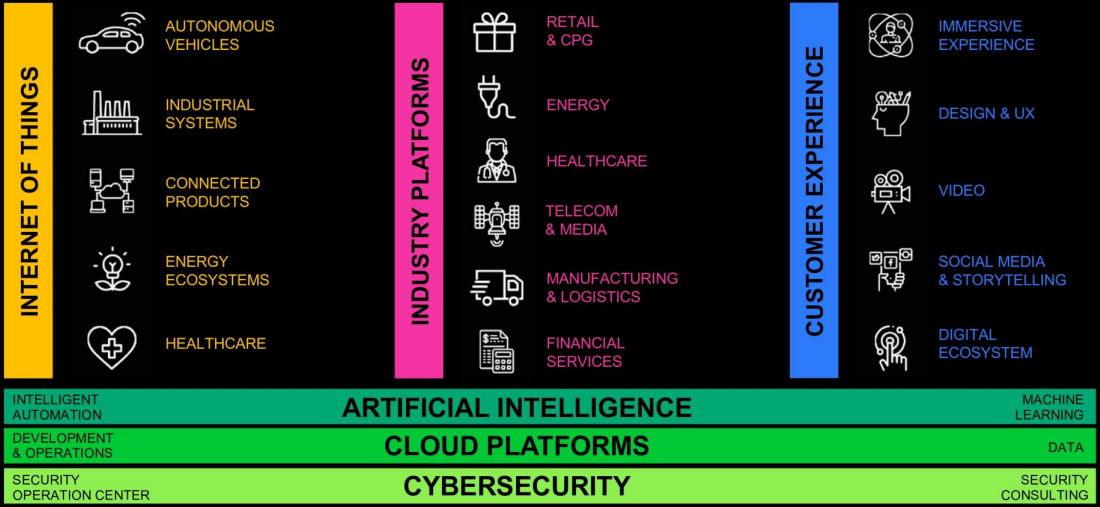
\includegraphics[width=0.75\linewidth]{images/bis2.png}
    \caption{Porter value chain}
\end{figure}

\paragraph*{Activity cycles}
Manufacturing involves continuous, iterative cycles that ensure efficiency and product quality. 
These cycles include:
\begin{enumerate}
    \item \textit{Development cycle}: focuses on designing and industrializing both products and production processes.
    \item \textit{Logistics cycle}: manages customer orders through:
        \begin{itemize}
            \item \textit{Procurement}: acquiring and handling materials, including reception, warehousing, and distribution to production plants.
            \item \textit{Production}: the physical transformation of raw materials into finished goods.
            \item \textit{Sales and distribution}: managing orders, external logistics, and post-sale services such as maintenance and customer support.
        \end{itemize}
\end{enumerate}

\subsection{Inter-functional information processes}
Inter-functional information processes play a key role in managing various aspects of production and operations within a company: 
\begin{enumerate}
    \item \textit{Order management process}: it manages the information regarding orders from order check in to post-sale services.
    \item \textit{Materials management process}: it manages the information regarding materials from outgoing orders towards suppliers to usage within transformation processes.
    \item \textit{Operations management process}: it manages the information regarding operations from materials dispatching to production plants to product delivery.
\end{enumerate}
\noindent These processes are interconnected across different products and divisions within the organization, making the information systems closely tied to the organizational structure. 
All production processes rely on the exchange of information across different functions. 
The use of inter-functional information extends beyond production and operations into planning and control processes. 
It also plays a vital role in administrative tasks.

\subsection{Production}
Companies may produce two types of goods: 
\begin{itemize}
    \item \textit{Standard production}: products have a finite set of predetermined features that can be changed to accommodate customer preferences. 
        In this case, companies produce according to a sales plan, before actual orders are received.
    \item \textit{Custom production}: products are designed according to customer requirements and then produced on demand.
\end{itemize}
\noindent While custom and standard production represent opposite ends of the production spectrum, there is a continuum between the two. 
Custom production is often seen in complex products, while standard production is associated with simpler goods. 
IT supports all production types, although its functionalities vary depending on the degree of customization or standardization in the production process.

\paragraph*{Product structure}
The product structure defines the hierarchical arrangement of components that make up a finished product. 
It ranges from individual components to larger product parts, outlining the relationships and dependencies between them.

\subsection{Information taxonomy}
Operational databases are organized to store various types of information that support the flow of activities within an organization. 
These can be categorized into three primary types: 
\begin{itemize}
    \item \textit{Transaction information}: describes the flow of operational activities, focusing on exchanges between different organizational units and external parties.
        It is the largest in terms of volumes. 
    \item \textit{Operation information}: details the objectives and expected results of operational activities. 
    \item \textit{Catalog information}: basic, static knowledge that exists independently of the flow of production activities. 
        It is quite complex and requires continuous updates and maintenance. 
        This information plays a key role in organizational learning.
\end{itemize}
\noindent Operations planning information is a key link between the operational and the executive portfolios.
Therefore, the level of detail of operational information is a driver of the efficiency of coordination inside an organization.
Operational information has intrinsic value as an organizational asset.
Its usefulness extends beyond internal operations, as it can sometimes be monetized or sold. 

\subsection{Information Technology integration}
Initially, IT functionalities were developed independently for each organizational function, without a comprehensive view of processes. 
The focus was on automating existing activities rather than supporting or re-engineering them to improve performance. 
Each function operated with separate data, and objectives were often misaligned, resulting in inefficiencies.

The traditional approach involved information being created at the start of a cycle and used later. 
However, to truly optimize organizational performance, a more proactive approach is needed. 
This involves using information at the executive level and integrating the various functions within an organization to create a unified view that enhances decision-making and operations.
There are two key approaches to IT integration:
\begin{itemize}
    \item \textit{Horizontal integration}: this refers to the integration of systems along the operating processes of an organization, specifically those that align with Porter's primary processes.
        This is done by the Computer Integrated Manufacturing (CIM), which is a system that supports the integration of manufacturing processes. 
    \item \textit{Vertical integration}: this focuses on connecting the operational portfolio with the executive portfolio. 
        This is done by the Material Requirements Planning (MRP), which ensures materials are available for production at the right time, helping optimize the production process and minimize waste.
\end{itemize}

\paragraph*{Computer Integrated Manufacturing}
CIM integrates various manufacturing processes. with the main objective of achieving an optimal scheduling and production resource management, which results in production efficiency. 
The main functionalities are: activities, workforce, plant, materials and quality management. 

\paragraph*{Materials Requirements Planning}
MRP is a production planning and inventory control system designed to manage manufacturing processes and ensure the availability of materials for production.
It emerged in the 1970s and 1980s with the aim of achieving flexibility and economies of scale through optimal planning. 
This is achieved with concurrent engineering (design and produce in parallel) and inside-out production processes (streamline production processes). 
MRP helps organizations achieve greater effectiveness by allowing them to respond more quickly to market demands while simultaneously benefiting from scale economies. 
    \section{Exercise 2}

An application permits the management of the bill of materials (BoM) of products. 
The BoM is the hierarchical description of a product in terms of the sub-products that comprise it. 
At each level but the last one, a product is associated with the components that make it, each with a quantity. 
The application allows the user to create BoMs.
A BoM is progressively assembled by attaching to a product its sub-products and specifying the number of units of sub-products that make one unit of the parent product. 
The editor accesses the HOME PAGE with the list of current BoMs and where s/he can create a new top level product and view the existing BOMs. 
The editor can add product-sub-products links to a product, modify the quantity of a product-sub-products link, delete a product or product-sub-products link. 
Products have an identifier, a name a description and a unit cost. 
An example of BoM is the following: 
\begin{figure}[H]
    \centering
    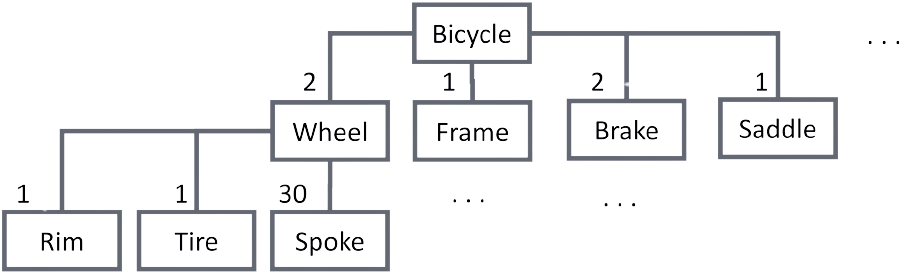
\includegraphics[width=1.0\linewidth]{images/BoM.png}
\end{figure}
The entity relationship model is the following:
\begin{figure}[H]
    \centering
    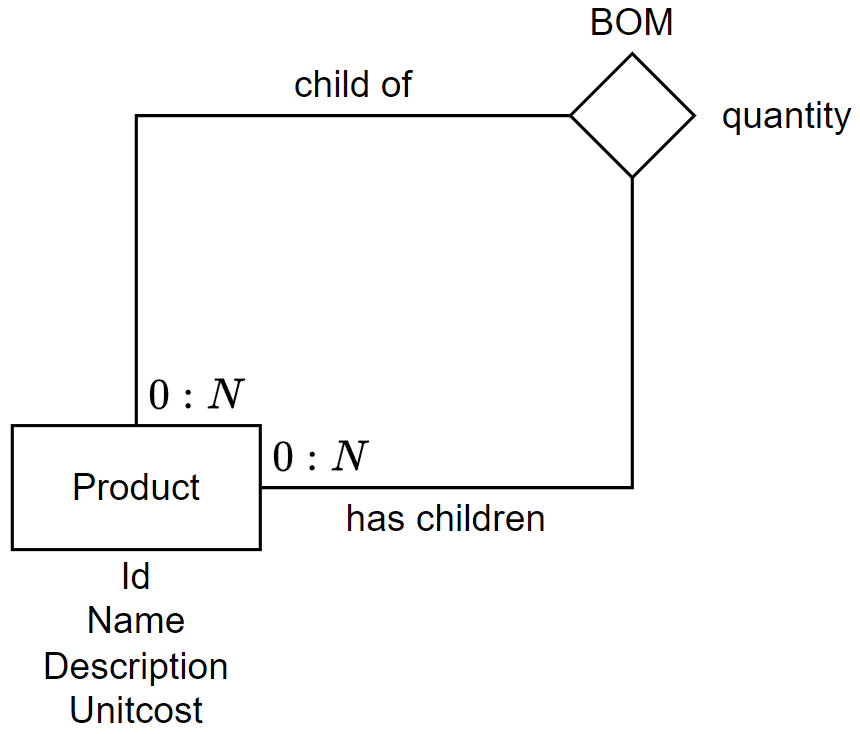
\includegraphics[width=0.5\linewidth]{images/e-r1.png}
\end{figure}
The relational schema DDL of the given database is: 
\begin{lstlisting}[style=SQL]
CREATE TABLE 'product' (
'id'            INT             NOT NULL AUTO_INCREMENT,
'unitcost'      INT             NOT NULL,
'name'          VARCHAR(45)     NOT NULL,
'description'   VARCHAR(45)     DEFAULT NULL,
PRIMARY KEY ('id')
) 
CREATE TABLE 'subparts' (
'father'        INT             NOT NULL,
'child'         INT             NOT NULL,
'quantity'      INT             NOT NULL,
PRIMARY KEY ('father','child'),
KEY 'childtoproduct_idx' ('child'),
CONSTRAINT 'childtoproduct' FOREIGN KEY ('child') REFERENCES 'product' ('id'),
CONSTRAINT 'fathertoproduct' FOREIGN KEY ('father') REFERENCES 'product' ('id')
)           
\end{lstlisting}
The relational model is: 
\begin{itemize}
    \item Product(\underline{id}, unitcost, name, description)
    \item Subparts(\underline{father}, \underline{child}, quantity)
\end{itemize}
Given the specifications, write the entity classes of the ORM mapping, including annotations for the attributes and for the relationships, fetch type of attributes and of relationships, and operation cascading policies for relationships (when not by default).

\subsection*{Solution}
Given the specifications write the entity classes of the ORM mapping, including annotations for the attributes and for the relationships, fetch type of attributes and of relationships, and operation cascading policies for relationships (when not by default). 
\begin{itemize}
    \item BoM: from father product to children product we have to use the annotations: 
        \begin{lstlisting}[style=Java]
@ManyToMany
        \end{lstlisting}
        From children product to father product we have to use these annotations: 
        \begin{lstlisting}[style=Java]
@ManyToMany
        \end{lstlisting}
        The owner of the relation is entity project. 
    \item 
\end{itemize}
The entity product is defined as:  
    \begin{lstlisting}[style=Java]
@Entity
@NamedQueries({
@NamedQuery(name = "BomProduct.findAll", query = "SELECT p FROM BomProduct p"),
@NamedQuery(name = "BomProduct.findAllTop", query = "SELECT p FROM BomProduct p WHERE p.fathers IS EMPTY") })

public class BomProduct implements Serializable {
    ...
    private static final long serialVersionUID = 1L;
    @Id @Column(name="id") @GeneratedValue(strategy = GenerationType.IDENTITY)
    private int id;
    private String description;
    private String name;
    private int unitcost;
    ...
    @ElementCollection(fetch = FetchType.EAGER)
    @CollectionTable(name = "subparts",joinColumns = @JoinColumn(name = "father"))
    @MapKeyJoinColumn(name = "child")
    @Column(name = "QUANTITY")
    private Map<BomProduct, Integer> subparts;

    @ManyToMany
    @JoinTable(name = "subparts",
            joinColumns = @JoinColumn(name = "child"),
            inverseJoinColumns = @JoinColumn(name ="father"))
    private List<BomProduct> fathers;
    ...            
}
    \end{lstlisting}
The better way is to make the many-to-many relationships with attributes a weak entity like in the following image. 
\begin{figure}[H]
    \centering
    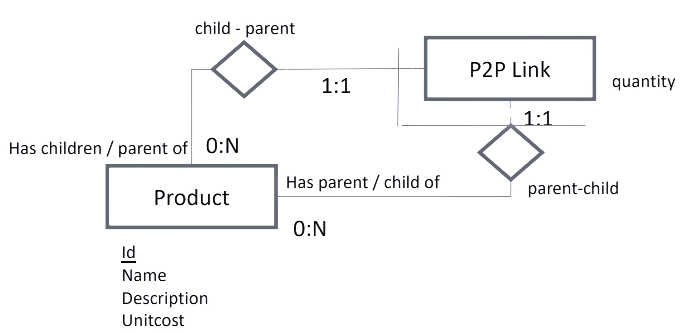
\includegraphics[width=0.5\linewidth]{images/BoMweak.png}
\end{figure}
The entity P2PLinkID is defined as:  
\begin{lstlisting}[style=Java]
@Embeddable
public class P2PLinkID implements Serializable {
    private static final long serialVersionUID = 1L;
    private int father;
    private int child;

    public P2PLinkID() { }

    public P2PLinkID(int father, int child) {
        super();
        this.father = father;
        this.child = child;
    }
    ...
}
\end{lstlisting}
The entity P2PLink is defined as:  
\begin{lstlisting}[style=Java]
@Entity
public class P2PLink implements Serializable {
    private static final long serialVersionUID = 1L;

    @EmbeddedId
    private P2PLinkID id;

    @ManyToOne
    @MapsId("father") // reference to the foreign key attribute
    @JoinColumn(name = "father")
    private BomProduct father;

    @ManyToOne
    @MapsId("child") // reference to the foreign key attribute
    @JoinColumn(name = "child")
    private BomProduct child;

    private int quantity;
    ...
}
\end{lstlisting}
The entity product is defined as:  
\begin{lstlisting}[style=Java]
@Entity
public class BomProduct implements Serializable {
    private static final long serialVersionUID = 1L;

    @Id @GeneratedValue(strategy = GenerationType.IDENTITY)
    private int id;
    private String description;
    private String name;
    private int unitcost;

    // getters setters and constructors

    @OneToMany(mappedby="father")
    private List<P2PLink> children;

    @OneToMany(mappedby="child")
    private List<P2PLink> fathers;
    ...
}
\end{lstlisting}

    \chapter{Exercise session IV}
    \section{Exercise one}

Consider the C program below, which is affected by a typical buffer overflow vulnerability.
\begin{verbnobox}[\verbarg]
#include <stdio.h>
#include <stdlib.h>
#include <string.h>

void vuln() {
    char buf[32];

    scanf("%s", buf);
    if (strncmp(buf, "Knight_King!", 12) != 0) {
        abort();
    }
}

int main(int argc, char** argv) {
    vuln();
}
\end{verbnobox}
\begin{enumerate}
    \item Assume that the program runs on the usual IA-32 architecture (32-bits), with the usual \texttt{cdecl} calling convention. 
        Also assume that the program is compiled without any mitigation against exploitation (ASLR is off, stack is executable, and stack canary is not present).
        Draw the stack layout when the program is executing the instruction at line seven, showing:
        \begin{itemize}
            \item Direction of growth and high-low addresses.
            \item The name of each allocated variable.
            \item The boundaries of frame of the function frames (\texttt{main} and \texttt{vuln}).
        \end{itemize}
        Show also the content of the caller frame.
    \item Write an exploit for the buffer overflow vulnerability in the above program. 
        Your exploit should execute the following simple shell code, composed only by four instructions: \texttt{0x12 0x34 0x56 0x78}.
        Write clearly all the steps and assumptions you need for the exploitation, and show the stack layout right after the execution of the \texttt{scanf()} during the program exploitation.
\end{enumerate}

\subsection*{Solution}
\begin{enumerate}
    \item To represent the stack layout described, we need to allocate space for the \texttt{buf} array, the saved EBP, and the saved EIP:
        \begin{figure}[H]
            \centering
            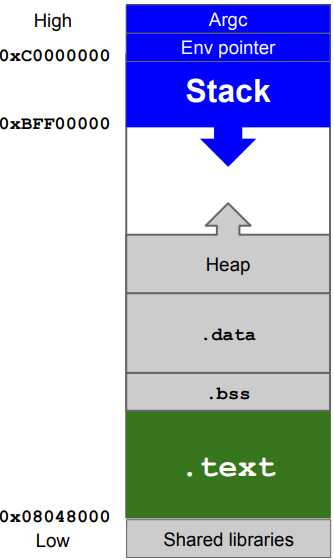
\includegraphics[width=0.5\linewidth]{images/stack.png}
        \end{figure}
    \item The stack in this case is: 
        \begin{figure}[H]
            \centering
            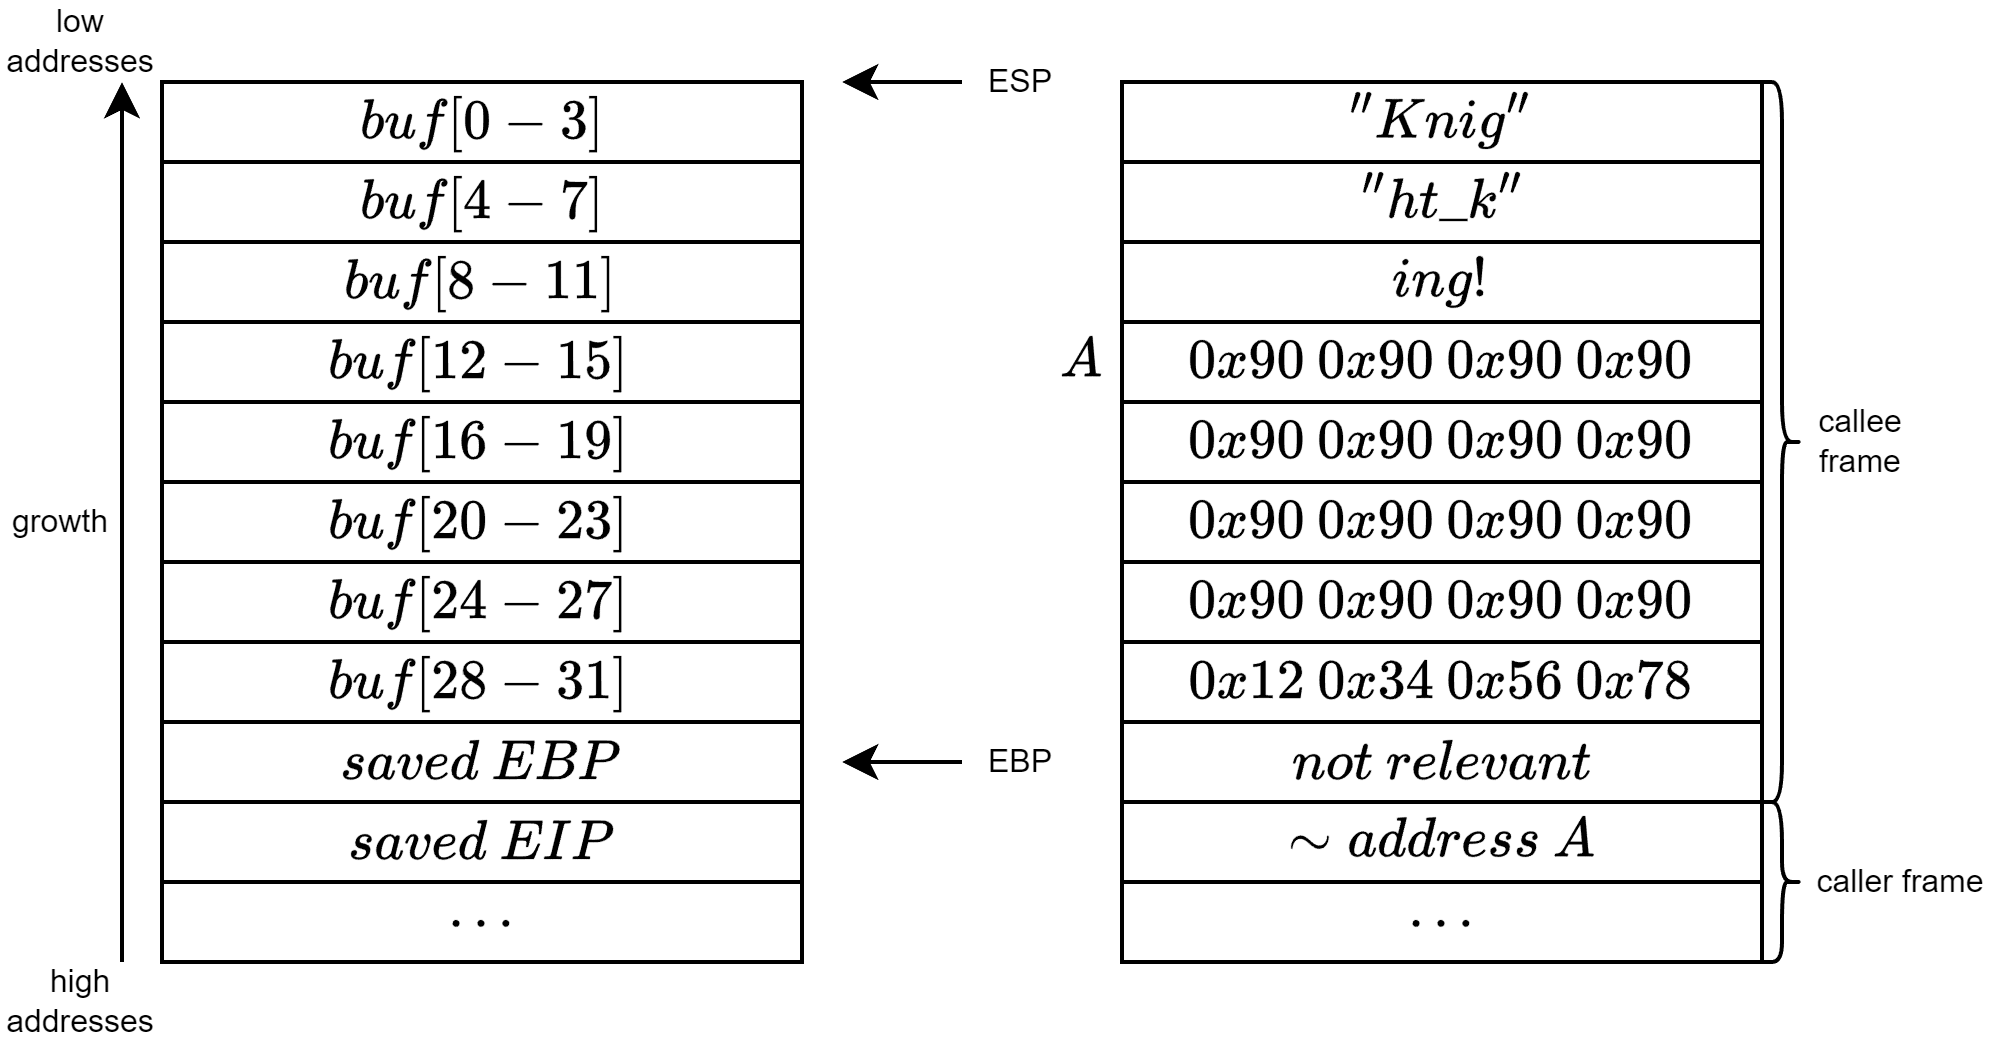
\includegraphics[width=0.75\linewidth]{images/stack1.png}
        \end{figure}
        In this layout:
        \begin{itemize}
            \item The first 16 bytes (four cells) are filled with no-operation instructions to avoid any unintended actions.
            The next 8 bytes (two cells) are reserved for the \texttt{buf} array.
            The following 4 bytes (one cell) are allocated for the saved EBP.
            The last 4 bytes (one cell) contain the address of the shell code.
        \end{itemize}
        The first twelve characters of \texttt{buf} are ensured to be different from "Knight\_King!" to avoid invoking \texttt{abort()}.
\end{enumerate}
    \section{Dependability principles}

Dependability is a critical consideration both during the design phase and during runtime operations.
During the design phase, it is essential to:
\begin{itemize}
    \item Analyze the system under development.
    \item Evaluate and measure its dependability properties.
    \item Make necessary modifications to the design as needed.
\end{itemize}
During runtime, the focus shifts to:
\begin{itemize}
    \item Detecting any malfunctions or failures that occur.
    \item Investigating and understanding the root causes of these issues.
    \item Taking appropriate reactive measures to address and mitigate the impact of the malfunctions.
\end{itemize}
Failures are commonplace in both the development and operational stages: while those in development should be averted, operational failures, being unavoidable due to the nature of system components, must be managed effectively. 
Design processes should factor in these potential failures to ensure that control and safety measures remain intact even when failures arise. 
Moreover, the effects of these failures should be predictable and deterministic rather than catastrophic.

Once upon a time, dependability was primarily a concern in safety-critical and mission-critical application domains like space exploration, nuclear facilities, and avionics. 
This was largely due to the significant cost associated with ensuring dependability, which was deemed acceptable only when absolutely necessary.
In non-critical systems, operational failures can lead to economic losses and damage to reputation, as seen in consumer products. 
However, in mission-critical systems such as satellites, automatic weather stations, surveillance drones, and unmanned vehicles, operational failures can result in serious or irreversible consequences for the mission at hand.
Safety-critical systems, on the other hand, pose a direct threat to human life if they fail during operation.
Examples include aircraft control systems, medical instrumentation, railway signaling, and nuclear reactor control systems.
    \section{Dependency}

To achieve higher performance within a given technology, it is crucial to extract more parallelism from the program. 
This involves detecting and resolving dependencies and scheduling instructions to maximize execution parallelism with the available resources.

Dependencies among instructions are key to determining the level of parallelism in a program. 
If two instructions are dependent on each other, they cannot execute simultaneously and must be executed sequentially or with limited overlap. 
There are three types of dependencies: name, data, and control dependencies.

\subsection{Name dependency}
A name dependency occurs when two instructions use the same register or memory location without any data flow between them.
There are two types of name dependencies between an instruction $i$ preceding instruction $j$:
\begin{itemize}
    \item \textit{Anti-dependence} (WAR): occurs when $j$ writes to a register or memory location that instruction $i$ reads. 
    \item \textit{Output dependence} (WAW): arises when both $i$ and $j$ write to the same register or memory location. 
\end{itemize}
Name dependencies differ from true data dependencies as there is no data flow between the instructions.

\paragraph*{Register Renaming}
If the names used in the instructions can be altered, the instructions do not conflict. 
Detecting dependencies through memory locations is more challenging since two addresses might refer to the same location but appear different. 
Register renaming is easier to implement and can be accomplished statically by the compiler or dynamically by the hardware.

\subsection{Data dependency}
Data dependencies can potentially create data hazards, but the actual hazard and the number of stalls required to eliminate it depend on the pipeline. 
There are three types of data hazards:
\begin{itemize}
    \item \textit{RAW hazards}: true data dependence.
    \item \textit{WAW hazards}: output dependence
    \item \textit{WAR hazards}: anti-dependence.
\end{itemize}
It is important to note that data dependencies are inherent to the program, while hazards are specific to the pipeline.

\subsection{Control dependency}
Control dependencies dictate the order of instruction execution, preserved by:
\begin{itemize}
    \item Executing instructions in program order to ensure that an instruction before a branch executes before the branch.
    \item Detecting control hazards to ensure that an instruction dependent on a branch is not executed until the branch direction is known.
\end{itemize}
While preserving control dependence is a simple way to maintain program order, it is not the most critical property that must be preserved for execution.

    \chapter{Exercise session V}
    \section{Introduction}

\begin{definition}[\textit{Integer linear programming problem}]
    An Integer linear programming (ILP) problem is an optimization problem of the form:
    \begin{align*}
        \min                      \:&\: c^Tx           \\
        \textnormal{such that }     &\: Ax = b         \\
                                    &\: x \in \mathbb{Z}^n
    \end{align*}  
\end{definition}
Additionally:
\begin{itemize}
  \item If $x_j \in \left\{ 0, 1 \right\} \: \forall, j$, the problem is called binary linear programming.
  \item If $\exists, i \text{ such that }x_i \notin \mathbb{Z}^n$, then the problem is called mixed integer linear programming.
\end{itemize}
Note that the integrality condition $x_i \in \mathbb{Z}$ is non-linear, as it can be expressed as $\sin(\pi x_j)=0$.
\begin{definition}[\textit{Linear relaxation}]
    Let $ILP$ be an ILP problem:
    \begin{align*}
        z_{ILP}:=\min                      \:&\: c^Tx           \\
        \textnormal{such that }     &\: Ax \leq b               \\
                                    &\: x \in \mathbb{Z}^n      \\
                                    &\: x \leq 0
    \end{align*}  
    Then the Linear Programming (LP) problem:
    \begin{align*}
        z_{LP}:=\max                      \:&\: c^Tx                    \\
        \textnormal{such that }             &\: Ax \leq b               \\
                                            &\: x \leq 0
    \end{align*}  
    is the linear (or continuous) relaxation of $ILP$.
\end{definition}
\begin{property}[Bounds of ILP solutions]  
    For any ILP with $\max$, the optimal solution is bounded by the optimal solution of the LP relaxation:
    \[ z_{ILP} \leq z_{LP} \]
  
    For any ILP with $\min$, the optimal solution is bounded by the optimal solution of the LP relaxation:
    \[ z_{ILP} \geq z_{LP} \]
\end{property}
The feasible region of any ILP is a lattice of points, either finite or infinite, depending on the type of problem.
By removing the integrality constraint, the ILP problem becomes an LP problem, and the optimal solution of the ILP problem isn't always the optimal solution of the LP problem.
\begin{figure}[H]
    \centering
    \begin{subfigure}[b]{0.495\textwidth}
        \centering
        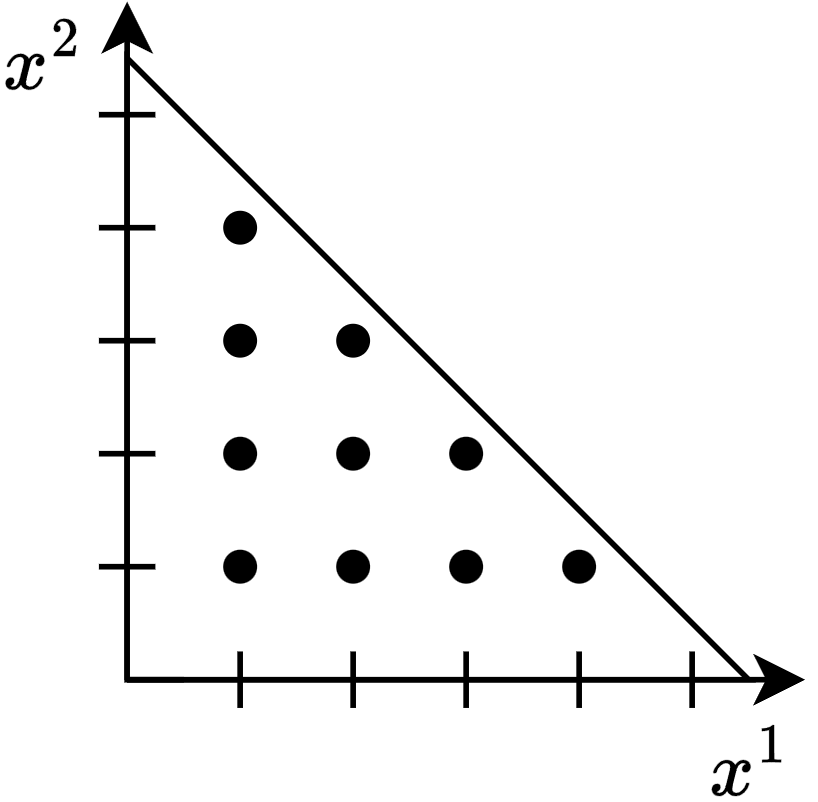
\includegraphics[width=0.4\linewidth]{images/ilp.png}
        \caption{Lattice of integer points}
    \end{subfigure}
    \begin{subfigure}[b]{0.495\textwidth}
        \centering
        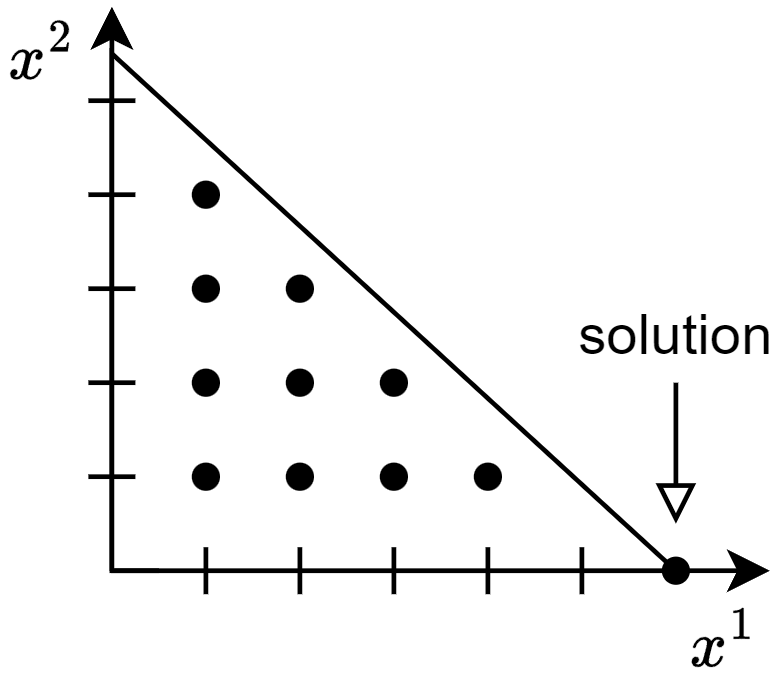
\includegraphics[width=0.4\linewidth]{images/ilp1.png}
        \caption{Relaxed lattice of integer points}
    \end{subfigure}
    \caption{Lattice of integer points}
\end{figure}
  
\subsection{Solutions of the ILP problem}
A viable approach to finding a solution to the ILP problem is to identify a solution to the LP problem and then round it to the nearest integer point.
If an optimal solution of the LP problem is an integer, it is also an optimal solution of the ILP problem. 
However, often the rounded optimal solutions of the LP are either:
\begin{itemize}
    \item \textit{Infeasible} solutions for the ILP.
    \item \textit{Useless} solutions for the ILP, as they are very different from an optimal solution of the ILP.
\end{itemize}
\begin{figure}[H]
    \centering
    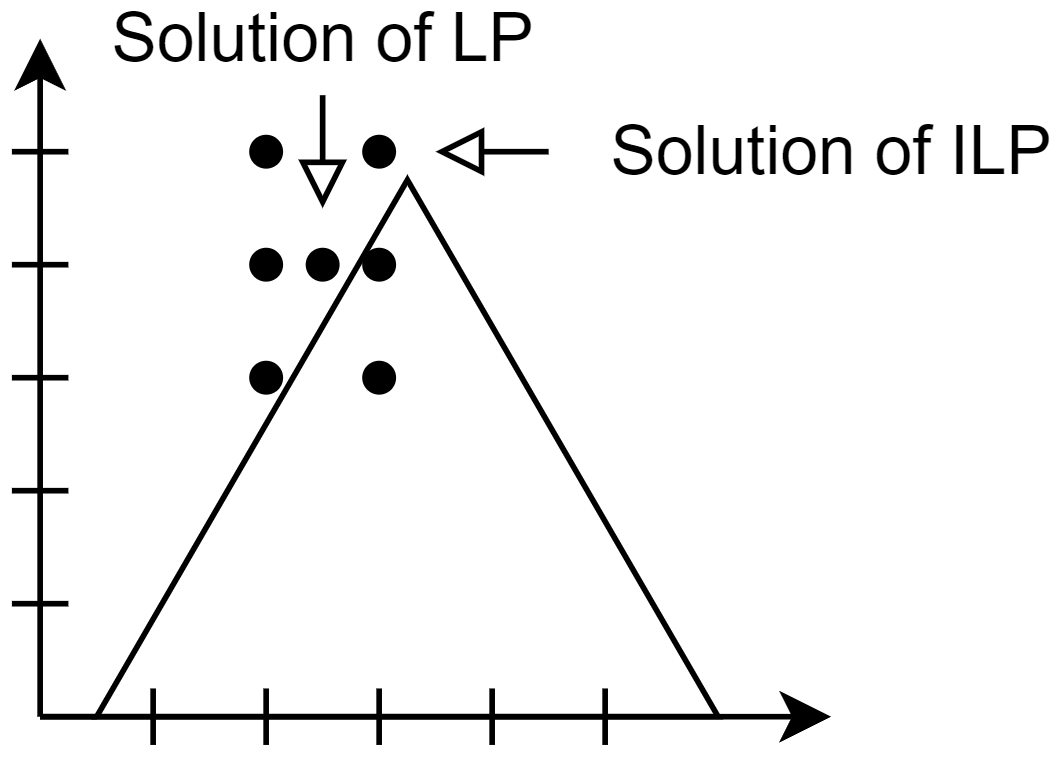
\includegraphics[width=0.25\linewidth]{images/ilp2.png}
    \caption{Solution of the LP relaxation of the ILP problem}
\end{figure}

\subsection{Solution of assignment and transportation problems}
Two crucial ILP problems, namely the assignment and transportation problems, have a solution that is the optimal solution of the LP relaxation.

\paragraph*{Assignment problem}
Given:
\begin{itemize}
    \item $m$ machines, $i = 1, \dots, m$
    \item $n$ jobs, $j = 1, \dots, n$, $n < m$
    \item $c_{ij}$ cost of assigning job $j$ to machine $i$
\end{itemize}
The goal is to determine an assignment of jobs to the machines to minimize the total cost. 
Each job must be assigned to exactly one machine, and each machine should have at least one job. 
The binary variables $x_{ij}$ represent the assignment, where:
\[ x_{ij} = 
\begin{cases}
    1 \quad & \text{if job } j \text{ is assigned to machine } i \\
    0 \quad & \text{otherwise}
\end{cases} \]
The assignment problem can be formulated as the following ILP problem:
\begin{align*}
\min        & \quad \sum_{i=1}^m \sum_{j=1}^n c_{ij} x_{ij}                                                      \\
\text{s.t.} & \quad \sum_{i=1}^{m} x_{ij} = 1 \quad \forall \, j \quad \text{at most one machine for each job}   \\
            & \quad \sum_{j=1}^{n} x_{ij} = 1 \quad \forall \, i  \quad \text{at least one job for each machine} \\
            & \quad x_{ij} \in \left\{ 0, 1 \right\} \quad \forall \, i, j
\end{align*}

\paragraph*{Transportation problem}
Given:
\begin{itemize}
\item $m$ productions plant, $i = 1, \dots, m$.
\item $n$ clients, $j = 1, \dots, n$, $n > m$ by assumption.
\item $c_{ij}$ cost of shipping one unit from plant $i$ to client $j$.
\item $p_i$ production capacity of plant $i$.
\item $d_j$ demand of client $j$.
\item $q_{ij} \geq 0$ quantity shipped from plant $i$ to client $j$.
\end{itemize}
The goal is to determine a transportation plan that minimizes the total costs while satisfying the production and demand constraints. 
The assumption is $\sum_{i=1}^m p_i \geq \sum_{j=1}^{n} d_j$.
Variables $x_{ij}$ represent the quantity shipped from plant $i$ to client $j$.

\paragraph*{Problems analysis}
In the assignment problem example, a forcing constraint is present, while the transportation problem introduces a constraint limiting the active number of variables.
\begin{definition}[\textit{Forcing constraint}]
    A constraint in the form: 
    \[ \displaystyle x \leq y\]
    is termed a forcing constraint if both $x$ and $y$ are binary variables.
\end{definition}
\begin{definition}[\textit{Constraint on binary variables}]
    A constraint of the form:
    \[ \displaystyle \sum_{i=1}^n x_i \leq 1 \]
    where all $x_i$ are binary variables, implies that at most one of the variables $x_i$ can be one. 
    Similarly, a constraint in the form: 
    \[ \displaystyle \sum_{i=1}^n x_i = 1 \]
    where all $x_i$ are binary variables, implies that exactly one variable $x_i$ must be one.
\end{definition}
The transportation problem illustrates that the optimal solution of the LP relaxation of the transportation problem is also the optimal solution of the ILP problem.
\begin{theorem}[Solution of the transportation problem]
    If in a transportation problem $p_i, \ d_{ij}, \ q_{ij}$ are all integers, all the basic feasible solutions (vertices) of its linear relaxation are integers.
\end{theorem}
\begin{proof}
    Let $A$ be an integer constraint matrix of size $\left( mn + n + m \right) \times \left( mn \right)$, where $a_{ij} \in \left\{ -1, 0, 1 \right\}$.
    The right-hand side vector $b$ is composed of integer elements.
    The optimal solution for the linear relaxation is:
    \[ x^\ast = \begin{bmatrix}
        B^{-1} b \\ 0
    \end{bmatrix}
    \qquad
    B^{-1} = \dfrac{1}{|B|}
    \begin{bmatrix}
        \alpha_{11} & \dots  & \alpha_{1n} \\
        \ldots      & \ldots & \ldots      \\
        \alpha_{m1} & \dots  & \alpha_{mn}
    \end{bmatrix}
    \]
    where $\alpha_{ij} = (-1)^{i+j} \det\left( M_{ij} \right)$, and $M_{ij}$ is the square submatrix obtained from $B$ by deleting the $i$-th row and the $j$-th column.
    Then:
    \begin{itemize}
        \item $B$ is integer $\Rightarrow$ $\alpha_{ij}$ is an integer.
        \item $\det\left( B \right) = \pm 1 \Rightarrow B^{-1}$ is an integer $\Rightarrow x^\ast$ is an integer.
        \item It can be shown that $A$ is totally unimodular, implying $\det\left( Q \right) = \{-1, 0, 1\}$ for any square submatrix $Q$ of $A$.    
    \end{itemize}
\end{proof}

\paragraph{Complexity of the ILP problem}
Most ILP problems are $\mathcal{NP}$-hard, meaning that there is no known algorithm capable of solving them and proving the solution's correctness in polynomial time. 
Various methods exist for finding optimal solutions, categorized as follows:
\begin{itemize}
    \item \textit{Implicit enumeration} methods: these aim to provide an exact solution, i.e., a global optimum. 
        Examples of this category include branch and bound and dynamic programming methods.
    \item \textit{Cutting planes} methods: these aim to provide an exact solution, i.e., a global optimum. 
    \item \textit{Heuristic} algorithms: these aim to provide an exact solution, i.e., a local optimum. 
        Greedy and local search algorithms fall into this category. 
\end{itemize}
    \section{Automatic Speech Recognition}

Automatic Speech Recognition (ASR) is the task of converting spoken language into written text. 
Traditionally, this problem was tackled using hand-engineered features and statistical models:
\begin{itemize}
    \item \textit{Feature extraction}: audio signals were first transformed into Mel-frequency cepstral coefficients (MFCCs) derived from Mel spectrograms.
    \item \textit{Modeling}: these features were then fed into Hidden Markov Models (HMMs) combined with Gaussian Mixture Models (GMMs) for sequence prediction.
\end{itemize}
\noindent However, the advent of Deep Learning has significantly changed the landscape of ASR.

A common approach using Convolutional Neural Networks (CNNs) involves classifying phonemes from raw audio or Mel spectrograms. This method, however, introduces several issues:
\begin{itemize}
    \item CNNs make predictions over fixed-size windows, but phonemes and words vary in duration.
    \item There's a need to determine how many windows correspond to each linguistic unit.
\end{itemize}
\noindent These limitations highlight the need for sequence models that can align input and output of different lengths.
A breakthrough in ASR came with encoder-decoder architectures, which can handle variable-length input and output sequences and learn temporal alignments without requiring fixed-size segmentation.

\paragraph*{Wav2vec}
Wav2Vec represents a significant advancement in ASR. 
It is a transformer-based model that operates directly on raw audio waveforms.
A convolutional frontend first extracts latent representations from the audio, which are then fed into a transformer encoder to capture temporal dependencies and contextual information. 
Importantly, Wav2Vec is trained in a self-supervised manner, enabling the use of large, unlabeled audio datasets.

\paragraph*{Whisper}
More recently, the Whisper model has achieved state-of-the-art performance in ASR. 
Unlike Wav2Vec, Whisper uses Mel spectrograms as its input representation and adopts an architecture inspired by Vision Transformers. 
Its training paradigm is weakly supervised and leverages vast amounts of diverse, multilingual data. 
This approach supports multiple languages and tasks, such as transcription, translation, and language detection, within a single unified model.

\subsection{Evaluation}
The performance of ASR systems is typically evaluated using two main metrics: Word Error Rate (WER) and Sentence Error Rate (SER).
WER quantifies the number of word-level substitutions, deletions, and insertions needed to transform the predicted transcription into the correct one, normalized by the number of words in the reference. 
SER, on the other hand, measures the proportion of sentences that contain at least one error, offering a complementary view of system performance at the sentence level.

\subsection{Advanced Automatic Speech Recognition}
Beyond general-purpose transcription, ASR systems can be adapted to improve accuracy for individual speakers. 
Speaker-specific variation, such as vocal tract length and pitch, can significantly affect recognition performance. 
Techniques such as vocal tract length normalization, which warps the frequency axis of the speech spectrum, help account for anatomical differences between speakers. 
Similarly, pitch normalization—particularly useful for recognizing children's speech. 
Another approach involves adapting a pre-trained acoustic model using a small amount of data from a new speaker to fine-tune the system for improved personalization.

An additional challenge in ASR is handling non-verbal and non-word sounds, which frequently occur in real-world audio. 
These include sounds like coughing, sighing, and environmental noises such as telephone rings or door slams. 
To accommodate these, special phonetic units can be defined, and corresponding placeholder words added to the model's lexicon and language model. 
Training data must include annotations for these special tokens to ensure the model can recognize and appropriately represent such sounds in the transcript.
    \section{Exercise 3}

A table STUDENT(StudID, SSN, LastName, FirstName, City, Faculty) has twenty thousand tuples and four indices with composite keys (attributes ordered left to right):
\begin{itemize}
    \item $IDX_1$(StudID, SSN, Faculty).
    \item $IDX_2$(LastName, FirstName, City).
    \item $IDX_3$(Faculty, City, LastName).
    \item $IDX_4$(Faculty, LastName, City).
\end{itemize}
Assuming uniform distribution of values for non-unique attributes, with:
\begin{itemize}
    \item $\text{val}(\text{LastName}) = 5000$.
    \item $\text{val}(\text{FisrtName}) = 1000$.
    \item $\text{val}(\text{City}) = 1000$.
    \item $\text{val}(\text{Faculty}) = 10$.
\end{itemize}
\begin{enumerate}
    \item Choose the best index for the following query:
        \begin{lstlisting}[style=SQL]
SELECT * 
FROM STUDENT
WHERE City = 'Milan' AND Faculty = 'Computer Science'
        \end{lstlisting}
    \item What if the query also had a selection on the LastName?
\end{enumerate}

\paragraph*{Solution}
\begin{enumerate}
    \item The where clause is a conjunction of supported predicates.
        We estimate the selectivity allowed by each of the available indexes, only considering the predicates mentioned in the where clause:
        \begin{itemize}
            \item $IDX_1$: there is no condition on StudID, so in this case we will have to follow all the pointer starting with StudID. 
                As a result it would force a full sequential scan of the table.
            \item $IDX_2$: there is no condition on LastName, so in this case we will have to follow all the pointer starting with LastName. 
                As a result it would force a full sequential scan of the table.
            \item $IDX_3$: the average number of candidate tuples is: 
                \[\dfrac{\left\lvert R \right\rvert }{\text{val}(\text{Faculty}) \cdot \text{val}(\text{City}) }=\dfrac{20000}{10 \cdot 1000}=2\]
                We excluded the LastName attribute since there is no restriction on it. 
            \item $IDX_4$: the average number of candidate tuples is: 
                \[\dfrac{\left\lvert R \right\rvert }{\text{val}(\text{Faculty}) \cdot \text{val}(\text{City}) }=\dfrac{20000}{10 \cdot 1000}=2\]
                We excluded the LastName attribute since there is no restriction on it. 
        \end{itemize}
        The best index is the more selective one, in this case we have that it is $IDX_3$. 
    \item We estimate the selectivity allowed by each of the available indexes, only considering the predicates mentioned in the where clause as before. 
        In this case we obtain 0.0004 tuples for both the third and the fourth indexes, but we choose the $IDX_4$ since it is more selective (LastName more selective than City)
\end{enumerate}

    \chapter{Exercise session VI}
    \section{Introduction}

Cloud Computing refers to a comprehensive, expansive system of computing, storage, and networking resources that are easily accessible to the public. 
These resources can be accessed through web service calls over the Internet, allowing for short- or long-term usage based on a pay-per-use model.

\subsection{Virtualization}
Virtualization involves partitioning and sharing hardware resources such as CPU and RAM among multiple virtual machines (VMs). 
A virtual machine monitor (VMM) oversees the allocation of physical resources to running VMs, ensuring performance isolation and security.

Without virtualization, software is closely tied to specific hardware, making it challenging to move or modify applications. 
Failures or crashes are typically isolated to individual servers, operating systems, and applications, resulting in low CPU utilization.

With virtualization, software and hardware become independent, offering greater flexibility with pre-built VMs. 
Operating systems and applications can be managed as unified entities, simplifying deployment and management.

The impact of virtualization on IT systems evolution includes server consolidation and the facilitation of cloud computing.

\paragraph*{Server consolidation}
Server consolidation involves migrating from physical to virtual machines. 
This process allows for seamless movement of virtual machines without disrupting the applications running inside. 
Workloads can be automatically balanced based on predefined limits and guarantees, ensuring efficient resource utilization and protecting servers and applications from component and system failures.
The advantages of server consolidation include:
\begin{itemize}
    \item Running different operating systems on the same hardware, leading to higher hardware utilization.
    \item Reduced hardware requirements, resulting in cost savings in acquisition and management (including human resources, power, and cooling), as well as promoting environmentally friendly practices (Green IT).
    \item Continued use of legacy software, such as running Windows applications on Linux machines through virtualization.
    \item Application independence from underlying hardware, providing flexibility and ease of maintenance.
\end{itemize}
    \section{Analytical Customer Relationship Management}

Analytical CRM focuses on leveraging customer data to derive actionable insights, enabling businesses to make informed decisions and enhance customer relationships. 
It encompasses various techniques and processes aimed at understanding customer behavior, predicting trends, and optimizing marketing strategies.

\subsection{Data mining}
Data mining involves the systematic analysis of large datasets to uncover hidden patterns, correlations, and insights that are critical for strategic business management. 
This process can be executed using a variety of techniques, ranging from traditional methods such as descriptive statistics, data visualization, and statistical correlations to more advanced approaches like machine learning algorithms.

These patterns must be presented in an intuitive and interpretable manner to ensure they can be effectively utilized by decision-makers. 
With the growing volume of operational data stored in corporate databases, data mining has become an essential tool for knowledge management, helping organizations unlock valuable insights embedded within their data.

\subsection{Customer profiling}
Customer profiling involves segmenting customers based on identifiable characteristics and behaviors, often facilitated by tools like loyalty cards or transaction histories. 
Customers can be categorized along multiple dimensions, including:
\begin{itemize}
    \item \textit{Loyalty}: analyzing purchasing habits to determine how frequently and consistently customers engage with the brand.
    \item \textit{Price Sensitivity}: assessing how responsive customers are to pricing changes or discounts.
    \item \textit{Lifestyle}: evaluating behavioral orientations across various dimensions, such as preferences, interests, and demographic factors.
\end{itemize}
\noindent Customer segmentation serves as the foundation for targeted marketing efforts. 
By identifying specific segments or combinations of segments, businesses can tailor promotions to align with the average characteristics of each group.
This approach not only enhances the effectiveness of marketing campaigns but also enriches the understanding of individual customer preferences.

\subsection{Campaign management}
Campaign management refers to the set of functionalities designed to support the planning, execution, and evaluation of marketing campaigns. 
A typical campaign lifecycle consists of four key phases, each with its associated tasks and objectives:
\begin{enumerate}
    \item \textit{Planning and budgeting}: defining campaign goals, target audiences, resource allocation, and financial constraints.
    \item \textit{Design}: developing campaign materials, messaging, and strategies to engage the intended audience effectively.
    \item \textit{Execution}: implementing the campaign across selected channels.
    \item \textit{Evaluation}: measuring campaign performance through key metrics.
\end{enumerate}


\end{document}